\documentclass[a4paper]{article}

\usepackage[hidelinks]{hyperref}
\usepackage{amssymb}
\usepackage{mathtools}
\usepackage{graphicx}
\usepackage{caption}
\usepackage{subcaption}

\begin{document}

\title{FEEG3003 Interim Report $-$ Learning and Exploiting Surrogate Models for Optimising the Structure of a Design}
\author{Alexander Atack $-$ 27745449}
\date{December 2018}
\maketitle

\section{Introduction}

\subsection{Aims \& objectives}

The core aim of this project is to imagine and implement an algorithm capable of learning to solve engineering design problems.
Such an algorithm should be sufficiently general that it can be trained to operate on a range of engineering environments,
and can cope with a variety of objective functions; specifically, it must be applicable to both discrete and continuously-valued objective functions.
Artificial neural networks (ANNs) and their properties as universal function approximators will be explored as a means of achieving this goal.

For the purposes of this report, a distinction is made between "intelligent" and "na\"ive" optimisation algorithms:
an intelligent algorithm utilises some domain knowledge $-$ which may be learned $-$ to explore the solution space in a directed way,
while na\"ive optimisation algorithms explore the solution space without using any learned domain knowledge, and may be iterative in nature.

If successful, the final deliverable of this project will be a description of an algorithm meeting these criteria,
possibly including a proof of the concept on a number of toy environments.
All code used for this project can be found at \url{https://github.com/aatack/IP}.

\subsection{Overview of structure}

The project will be split into three main phases, each of which will attempt to approximate a particular function:
\begin{enumerate}
  \item Train an articial neural network, referred to as the discriminator \textbf{D}, to predict the probability that a solution satisfies some set of constraints.
  $$\mathrm{\textbf{D}} : (\mathrm{constraints}, \mathrm{solution}) \mapsto p(\mathrm{constraints \; satisfied} \; | \; \mathrm{solution})$$
  It is assumed that both the solution and set of constraints can be represented as a tensor of real values.
  \item Invert the discriminator to produce a generative model \textbf{G} parameterised by a set of constraints
  which is capable of sampling from the space of solutions which are likely to satisfy that set of constraints.
  $$\mathrm{solution} \sim \mathrm{\textbf{G}}(\mathrm{constraints}) $$
  Instead of using data to train the generator, the discriminator will be used to provide gradients for backpropagation;
  intuitively, this is similar to training the generator on the laws governing the environment rather than specific examples of solutions in that environment.
  \item Find a way to map a solution space which cannot be represented by a fixed-size tensor of real values to and from a vector representation
  so that it can be optimised using the functions learned in the previous phases.
  This will involve learning a function \textbf{L} that maps some arbitrary data structure to a $n$-dimensional latent space.
  $$\mathrm{\textbf{L}} : \mathrm{design} \mapsto \mathbb{R}^n$$
  Options for doing this include vector embeddings, recursive neural networks (RNNs), or LSTM networks.

\end{enumerate}

\section{Literature Review}

\subsection{Na\"{i}ve optimisation techniques}

A number of algorithms exist for finding the minimum of a scalar or vector function.
Many of these are gradient descent algorithms \cite{ruder17} which use information about the local gradient of the objective function
to iteratively minimise error.
Because the gradient is used to update the estimate, these algorithms often fail to converge quickly on problems where the error surface is very flat.
Algorithms such as RMSProp \cite{hinton17} and Adam \cite{kingma17} have been developed to overcome this, but still fail to converge if the objective function is discretised.

Gradient-free optimisation algorithms such as particle swarm optimisation \cite{kennedy12} solve this problem for environments of small dimensionality
by rapidly exploring the state space, then focusing on areas which give good results.
But the expected runtime of such algorithms drop off exponentially as the dimensionality of the state space increases.

Genetic algorithms \cite{carr14}, sometimes considered to fall under the umbrella of machine learning, are a certain kind of optimisation algorithm
which are both gradient-free and stochastic.
They are still not intelligent optimisation algorithms, however, because they only adapt solutions to constraints, and do not adapt their overall strategy to different environments.

\subsection{Artificial neural networks}

At times, the function being optimised will be a particular parameterisation of a specific type of function.
In this case, there may exist an analytical solution for the optimum which is a function of the parameters.
It might therefore be expected that a universal function approximator could be able to learn this mapping.

ANNs are known to be universal function approximators \cite{hornik91}.
In particular, deep neural networks (DNNs) \cite{liang17} are capable of approximating highly intractable functions to within a reasonable degree of accuracy.
One limiting factor of the performance of ANNs and DNNs is the quantity of data available.
While larger networks with more capacity are able to learn more complex mappings, they also run a higher risk of overfitting, \cite{caruana01},
a problem which is exacerbated in situations where the amount of training data may be limited.

Regularisation techniques have been developed \cite{goodfellow16, srivastava14, ioffe15, li18} to prevent the overfitting of neural networks.
These techniques generally rely on reducing the reliance of the network on singular large weights:
this makes it more difficult for the network to detect and memorise individual data points, thereby forcing it to learn a more generic mapping.
Bayesian neural networks \cite{giryes16} view the problem of finding the network weights through a Bayesian lens rather than a frequentist one.
A Bayesian network will sample its weights from a probability distribution, with weight vectors more likely to be sampled if they are
more likely to explain the dataset seen by the network during its training.
This can boost network performance when only a small number of examples are available, and can give an idea of the uncertainty
of the network by performing multiple forward passes and seeing how closely the network output from each pass agree with one another.

Adding noise to the network's input vector \cite{zur09} has also been shown to decrease overfitting and increase the generality of the network's estimates,
especially for applications where the available data are sparsely spread throughout the state space.
The effect of adding noise to the input vector is to simulate a much greater number of data points, but this method does
assume that data points which are nearby in the state space will produc similar outputs.
The level of noise is another hyperparameter which must be optimised: too little noise will have no effect on overfitting,
while too much noise will make it impossible for the network to distinguish between noise and genuine information, causing a drop in accuracy.

\subsection{Function inversion}

As well as approximating functions mapping between two sets, ANNs are capable of learning the inversion of an existing function.
Promising results have been obtained using standard ANNs to invert sometimes intractable functions in image processing,
for uses such as image deblurring \cite{nah18} and colourisation \cite{nguyen16}.

Autoencoders are an unsupervised learning method often used to pretrain layers of neural networks that will later be used for supervised learning \cite{rumelhart86},
in doing so training an encoder $f(x)$ and a decoder $f^{-1}(x)$.
This can be used to extract the more important latent features of the input space, or remove noise from corrupted data \cite{vincent08}.
When used for pretraining, the decoder is normally thrown away; but if the encoding function $f(x)$ is already know, the autoencoder architecture can be used to approximate its inverse.

Other architectures have been proposed which perform the same task as a traditional autoencoder, but train a generative model to do so.
Variational autoencoders (VAEs) are models which allow sampling from the latent space by parameterising a probability distribution over the latent space \cite{kingma14},
indicating which latent variables are most likely to explain the visible data.
The most common use for this is in learning a more robust latent mapping for a dataset, but the method could be adapted to create a generative model that inverts a many-to-one function.

A common problem faced by traditional autoencoders is that not every point in the latent space has a meaningful equivalent in the state space.
A regularisation term is imposed on a VAE in the $\beta$-VAE architecture \cite{higgins16} that encourages a higher standard deviation in the probability distribution over the latent space.
The effect of this is that input data may be mapped to a greater variety of regions in the latent space,
and therefore a greater proportion of the latent space will have a meaningful inverse mapping.

\subsection{Adversarial algorithms}

More recently, algorithms have been designed to train generative models using two competing networks in a minimax game.
The most common adversarial networks, generative adversarial networks (GANs), can be trained to sample from an arbitrary distribution \cite{goodfellow14, horger18}.
These have been successfully applied to a range of problems, including image resolution upscaling \cite{ledig17} and creating cross-domain transfer functions \cite{zhu18}.
Such applications could be useful in using GANs to sample from a space of viable solutions, if the space can be parameterised according to the relevant constraints.

Some research has also been done into the use of GANs to invert functions \cite{anirudh18};
while autoencoders can also accomplish this task and are generally considered to be easier to train \cite{bang18},
the generative nature of GANs is appealing considering that any given engineering problem may have more than one solution.

\subsection{Representation learning}

All of the neural network architectures discussed so far require the input data to be presented in the form of a fixed-size tensor of real values.
While many practical data structures can be meaningfully encoded in this form, many engineering problems can have solutions which are discrete,
unbounded, or otherwise not easily represented by a tensor of real values.

Long short-term memory networks (LSTMs) \cite{hochreiter97} are stateful networks which collate information over a linear series of tensors into a fixed-size memory.
At each time step, another item from the series is viewed by the network, and it decides which information to keep, and which to forget.
If trained properly, the memory tensor at the end is a fixed-size representation of the important features of the list.

Recursive neural networks merge information about pairs of objects, allowing the construction of representations of tree-like data structures \cite{socher11}.
As such, they are frequently used to parse sentences in natural language processing, though this technique can be applied to other trees as well.
Like with LSTMs, because the information capacity of the final state tensor is finite, the network is forced to either generalise, or forget unimportant information.

Some data structures, known as tokens, cannot be represented by real values and do not consist of sub-elements that can.
The prime example of these data structures are words; each word carries meaning but the meaning of each word is encoded in the understanding of the people using them.
Vector space models represent tokens as points in a vector space, and some methods have been developed for embedding tokens in this vector space.
One method commonly used is \emph{word2vec} \cite{mikolov13}, which embeds words into a dense vector space, though the same principle
has been adapted for use on tokens other than words \cite{le14}.

\section{Current Progress}

Progress so far has focused on the completion of the first phase of the project.
The goals are to prove that a discriminator can practically be trained on a number of engineering environments,
and to investigate any trends in network architecture that might produce better results.

\subsection{Environment design}

Two different engineering environments were used to the first phase.

The state space of the first environment, referred to as the circle environment, is a 6-dimensional hypercube on $(-1, 1)^6$.
Its state variables represent two circles, each of which has its $x$- and $y$-coordinates controlled, as well as its radius.
The first circle is considered to be the constraint, while the second is considered to be the solution, or design;
if the constraint circle is partially or fully occluded by the solution circle, the solution satisfies the constraint.
So the objective function is:
\[
  f(x)= 
\begin{dcases}
  1, & \text{if } (x_c - x_s)^2 + (y_c - y_s)^2 \leq (r_c + r_s)^2\\
  0, & \text{otherwise}
\end{dcases}
\]
While simple and very abstract, this environment should test that the discriminator is able to cope with discrete objective functions.

The state space of the second environment, referred to as the bridge environment, is a $h \times w$ matrix,
in which the value each cell represents the weight of a square element of a 2-dimensional bridge and is constrained to be between $0$ and $1$.
Each block bears a certain amount of load, and will break if the load it bears is greater than its weight.
If any blocks fail, the bridge is deemed invalid.
Each block takes a proportion of its own weight as load, and then propagates a proportion of its own weight to the block below it and $n$ blocks to either side of that one;
its load is distributed to each of the supporting blocks, distributed according to how much each supporting block weighs, with heavier blocks taking more load.
The load of each block is calculated row by row, starting from the top row and moving downwards.

As well as being structurally sound, the bridge is required to adhere to a maximum and minimum weight for each block.
The allowable weight range for each block is specified by the constraint, which takes the form of a $h \times w \times 2$ tensor.
This lets certain exclusion zones to be defined, in which all blocks must have a weight of, say, less than $0.01$;
inclusion zones can also be defines, in which all blocks must weigh at least a certain amount.

\begin{figure}
\centering
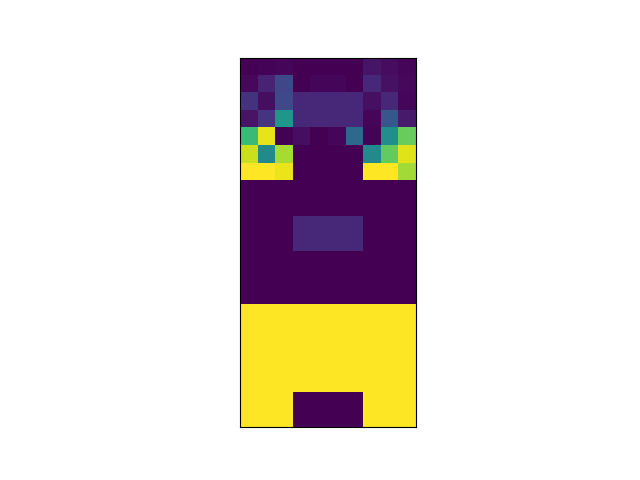
\includegraphics[scale=0.6]{../../figures/validbridges/valid_bridge_9.png}
\caption{
  An example of a valid bridge.
  Brighter pixels are blocks with a greater weight.
  The image is split vertically into thirds:
  the top one represents the bridge design,
  the middle one represents the block weight lower bounds,
  while the bottom one represents the block upper bounds.}
\label{fig:validBridgeExample}
\end{figure}

An example of a valid bridge design is shown in Figure \ref{fig:validBridgeExample}.

\subsection{Training discriminators}

Due to the universality of ANNs \cite{hornik91} it is theoretically possible for a network to classify solutions that satisfy constraints and those that do not.
Some experiments were run on the circle environment to see whether this is practically possible.
At first, no limit was placed on the number of data points availabe; instances were generated procedurally as needed by the network
by uniformly sampling from the state space.

The discriminator itself consisted of a standard MLP with six input nodes, one sigmoid output node, and a single hidden layer of $n$ ReLU-activated nodes.
Training examples $x_i$ were fed to the network, then gradients were calculated against $y_i \in 0, 1$ where $0$ represented a solution
that did not satisfy the constraint $-$ the circles did not overlap $-$ and $1$ represented a solution that did.

\begin{figure}
\centering
  \begin{subfigure}[a]{.8\linewidth}
    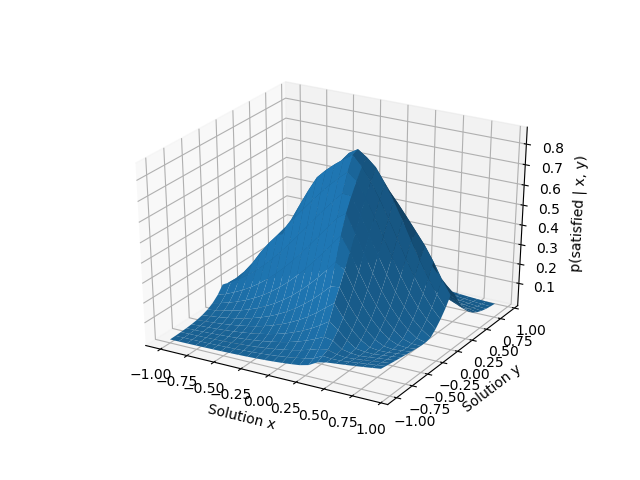
\includegraphics[width=.8\linewidth]{../../figures/artificial-discriminator-predicted-objective-function-4-hidden-nodes.png}
    \caption{$n = 4$.}
  \end{subfigure}
  \begin{subfigure}[a]{.8\linewidth}
    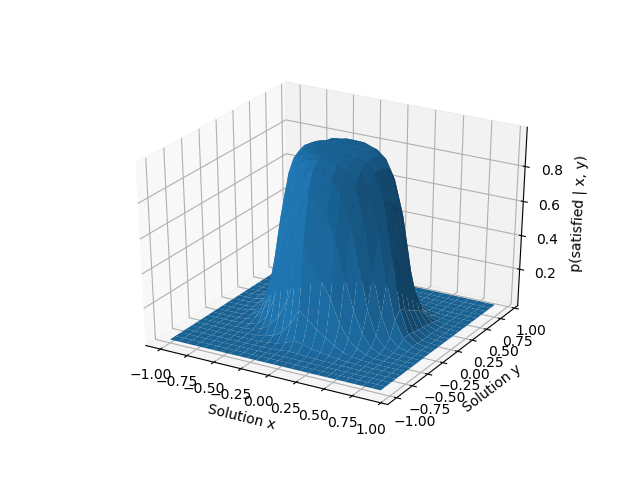
\includegraphics[width=.8\linewidth]{../../figures/artificial-discriminator-predicted-objective-function-16-hidden-nodes.png}
    \caption{$n = 16$.}
  \end{subfigure}
  \begin{subfigure}[a]{.8\linewidth}
    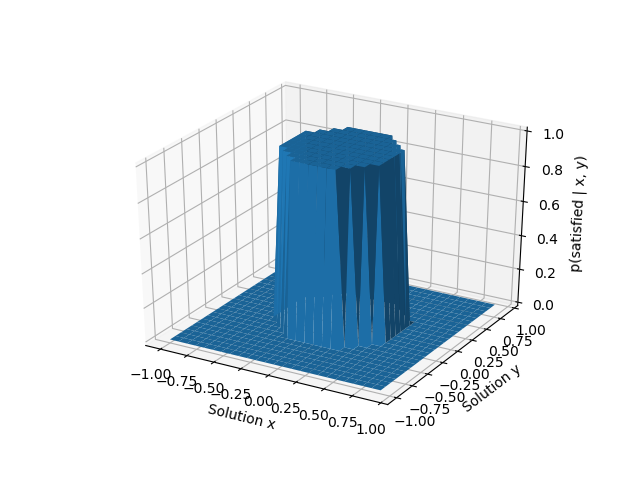
\includegraphics[width=.8\linewidth]{../../figures/artificial-discriminator-true-objective-function.png}
    \caption{Ground truth.}
  \end{subfigure}
  \caption{
    Network output when varying the $x$- and $y$-coordinates of the solution circle in the circles environment,
    for $n=4$ hidden nodes, $n=16$ hidden nodes, and for the ground truth objective function.
  }
\label{fig:artificialDiscriminator}
\end{figure}

In Figure \ref{fig:artificialDiscriminator}, the output of the discriminator is plotted while varying the $x$- and $y$-coordinates
of the solution circle, while holding all other parameters constant.
As expected, more hidden nodes draws the function approximated by the discriminator closer to the real objective function.
Even with only four hidden nodes, however, the network has managed to learn the general shape of the objective function.
While the edges are not as sharply defined, the network correctly predicts that the probability that the solution satisfies
the constraint is highest when the solution circle is centred on the constraint circle, and includes increasing
uncertainty in its classification as the candidate solution moves away from the most obvious one.

\subsection{Regularisation methods}



\subsection{Hyperparameter tuning}

\section{Future Work}

\subsection{Training generators}

\subsection{Sampling from nonlinear topologies}

\begin{thebibliography}{999}

\bibitem{ruder17}
  S. Ruder,
  \emph{An overview of gradient descent optimization algorithms}.
  arXiv:1609.04747v2 [cs.LG],
  15 Jun 2017.

\bibitem{hinton17}
  G. Hinton, N. Srivastava, K. Swersky,
  \emph{Overview of mini-batch gradient descent}.
  University of Toronto
  [online lecture notes]
  2017.
  \url{https://www.cs.toronto.edu/~tijmen/csc321/slides/lecture_slides_lec6.pdf}.

\bibitem{kingma17}
  D.P. Kingma, J.L. Ba,
  \emph{Adam: A Method for Stochastic Optimization}.
  arXiv:1412.6980v9 [cs.LG],
  30 Jan 2017.

\bibitem{kennedy12}
  J. Kennedy, R. Eberhart,
  \emph{Particle Swarm Optimisation}.
  Washington, DC,
  2012.

\bibitem{carr14}
  J. Carr,
  \emph{An Introduction to Genetic Algorithms}
  [online].
  May 16, 2014,
  \url{https://www.whitman.edu/Documents/Academics/Mathematics/2014/carrjk.pdf}.

\bibitem{hornik91}
  K. Hornik,
  \emph{Approximation Capabilities of Multilayer Feedforward Networks}.
  Neural Networks,
  1991,
  Volume 4,
  Issue 2,
  Pages 251-257.

\bibitem{liang17}
  S. Liang, R. Srikant,
  \emph{Why Deep Neural Networks for Function Approximation?}.
  arXiv:1610.04161v2 [cs.LG],
  3 Mar 2017.

\bibitem{caruana01}
  R. Caruana, S. Lawrence, L. Giles,
  \emph{Overfitting in Neural Nets: Backpropagation, Conjugate Gradient, and Early Stopping}.
  NIPS,
  2001.

\bibitem{goodfellow16}
  I. Goodfellow, Y. Bengio, A. Courville,
  2016.
  \emph{Deep Learning}
  [online],
  MIT Press.
  \url{http://www.deeplearningbook.org/contents/regularization.html}.

\bibitem{srivastava14}
  N. Srivastava, G. Hinton, A. Krizhevsky, I. Sutskever, R. Salakhutdinov,
  \emph{Dropout: A Simple Way to Prevent Neural Networks from Overfitting}.
  Journal of Machine Learning Research, 
  15 (Jun): 1929-1958, 2014.

\bibitem{ioffe15}
  S. Ioffe, C. Szegedy,
  \emph{Batch Normalization: Accelerating Deep Network Training by Reducing Internal Covariate Shift}.
  arXiv:1502.03167v3 [cs.LG],
  2 Mar 2015.

\bibitem{li18}
X. Li, S. Chen, X. Hu, J. Yang,
\emph{Understanding the Disharmony between Dropout and Batch Normalization by Variance Shift}.
arXiv:1801.05134v1 [cs.LG],
16 Jan 2018.

\bibitem{giryes16}
  R. Giryes, G. Sapiro, A.M. Bronstein,
  \emph{Deep Neural Networks with Random Gaussian Weights: A Universal Classification Strategy?}.
  arXiv:1504.08291v5 [cs.NE],
  14 Mar 2016.

\bibitem{zur09}
  R.M. Zur, Y. Jiang, L.L. Pesce, K. Drukker,
  \emph{Noise injection for training artificial neural networks: A comparison with weight decay and early stopping}.
  Med Phys.
  2009 Oct;
  36(10): 4810–4818.

\bibitem{nah18}
  S. Nah, T.H. Kim, K.M. Lee,
  \emph{Deep Multi-scale Convolutional Neural Network for Dynamic Scene Deblurring}.
  arXiv:1612.02177v2 [cs.CV],
  7 May 2018.

\bibitem{nguyen16}
  T. Nguyen, K. Mori, R. Thawonmas,
  \emph{Image Colourization Using a Deep Convolutional Neural Network}.
  ASIAGRAPH Conference,
  2016.

\bibitem{rumelhart86}
  D.E. Rumelhart, G. Hinton, R.J. Williams,
  \emph{Learning internal representations by error propagation}.
  Parallel Distributed Processing,
  Vol 1: Foundations,
  MIT Press,
  Cambridge, MA,
  1986.

\bibitem{vincent08}
  P. Vincent, H. Larochelle, Y. Bengio, P. Manzagol,
  \emph{Extracting and Composing Robust Features with Denoising Autoencoders}.
  Universit\'e de Montr\'eal,
  2008.

\bibitem{kingma14}
  D.P. Kingma, M. Welling,
  \emph{Auto-Encoding Variational Bayes}.
  arXiv:1312.6114v10 [stat.ML],
  1 May 2014.

\bibitem{higgins16}
  I. Higgins, L. Matthey, A. Pal, C. Burgess, X. Glorot, M. Botvinik, S. Mohamed, A. Lerchner,
  \emph{beta-VAE: Learning Basic Visual Concepts with a Constrained Variational Framework}.
  ICLR,
  04 Nov 2016.

\bibitem{goodfellow14}
  I. Goodfellow, J. Pouget-Abadie, M. Mirza, B. Xu, D. Warde-Farley, S. Ozair, A. Courville, Y. Bengio,
  \emph{Generaitve Adversarial Nets}.
  arXiv:1406.2661v1 [stat.ML],
  10 Jun 2014.

\bibitem{horger18}
  F. Horger, T. W\"urfl, V. Christlein, A. Maier,
  \emph{Deep Learning for Sampling from Arbitrary Probability Distributions}.
  arXiv:1801.04211v2 [cs.LG],
  10 Jul 2018.

\bibitem{ledig17}
  C. Ledig, L. Theis, F. Husz\'ar, J. Caballero, A. Cunningham, A. Acosta, A. Aitken, A. Tejani, J. Totz, Z. Wang, W. Shi,
  \emph{Photo-Realistic Single Image Super-Resolution Using a Generative Adversarial Network}.
  arXiv:1609.04802v5 [cs.CV],
  25 May 2017.

\bibitem{zhu18}
  J. Zhu, R. Park, P. Isola, A.A. Efros,
  \emph{Unpaired Image-to-Image Translation using Cycle-Consistent Adversarial Networks}.
  arXiv:1703.10593v6 [cs.CV],
  15 Nov 2018.

\bibitem{anirudh18}
  R. Anirudh, J.J. Thiagarajan, B. Kailkhura, T. Bremer,
  \emph{An Unsupervised Approach to Solving Inverse Problems using Generative Adversarial Networks}.
  arXiv:1805.07281v2 [cs.CV],
  4 Jun 2018.

\bibitem{bang18}
  D. Bang, H. Shim,
  \emph{MGGAN: Solving Mode Collapse using Manifold Guide Training}.
  arXiv:1804.04391v1 [cs.CV],
  12 Apr 2018.

\bibitem{hochreiter97}
  S. Hochreiter, J. Schmidhuber,
  \emph{Long Short-Term Memory}.
  Neural Computation,
  Volume 9 Issue 8,
  15 November 1997.

\bibitem{socher11}
  R. Socher, C.C. Lin, A.Y. Ng, C.D. Manning,
  \emph{Parsing Natural Scenes and Natural Language with Recursive Neural Networks}.
  Stanford University,
  2011.

\bibitem{mikolov13}
  T. Mikolov, K. Chen, G. Corrado, J. Dean,
  \emph{Efficient Estimation of Word Representations in Vector Space}.
  arXiv:1301.3781v3 [cs.CL],
  7 Sep 2013.

\bibitem{le14}
  Q. Le, T. Mikolov,
  \emph{Distributed Representations of Sentences and Documents}.
  arXiv:1405.4053v2 [cs.CL],
  22 May 2014.

% Insert here

\bibitem{sigmund01}
  O. Sigmund,
  \emph{A 99 line topology optimization code written in Matlab}.
  Struct Multidisc Optim 21,
  120-127,
  2001.

\bibitem{luo18}
  R. Luo, F. Tian, T. Qin, E. Chen, T. Yiu,
  \emph{Neural Architecture Optimization}.
  arXiv:1808.07233v4 [cs.LG],
  31 Oct 2018.

\bibitem{yu18}
  Y. Yu, T. Hur, J. Jung, I.G. Jang,
  \emph{Deep learning for determining a near-optimal topological design without any iteration}.
  Springer Nature,
  2018.

\end{thebibliography}

\end{document}
